
% Theory part goes here %

% for numerated formulas
\newcommand{\formula}[3]
{
    \noindent#1\\[0.1cm]
    \begin{equation}\label{#2}
        #3
    \end{equation}
}

% for in-text math formulas
\newcommand{\mth}[1]
{
    \begin{math}
        #1
    \end{math}
}

% for rus letters in indexes
\newcommand{\ruB}[1]
{
    _{\text{#1}}
}

\section{Экспериментальная установка}

\begin{figure}[h!]
    \center{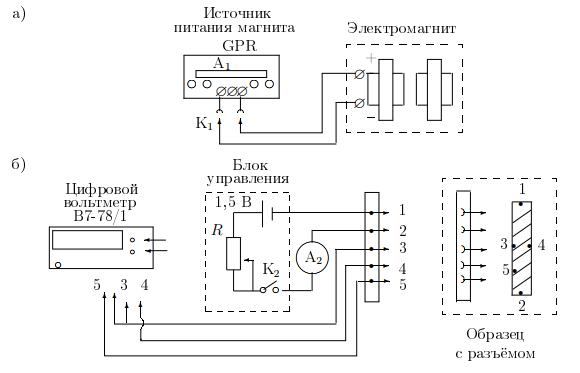
\includegraphics[width = 0.7\textwidth]{2.png}}\\
    \textit{Рис. 1: Схема экспериментальной установки}
\end{figure}
Схема для измерения ЭДС Холла представлена на рисунке 1. В зазоре электромагнита создаётся постоянное магнитное поле, величину которого можно менять регуляторами источника питания электромагнита.

Образец из легированного германия, смонтированный в специальном держателе, подключается к источнику питания. При замыкании К$_2$ вдоль длинной стороны образца течёт ток, величина которого регулируется реостатом $R$ и измеряется миллиамперметром. В образце, помещённом в зазор, возникает разность потенциалов $U_{34}$, которая измеряется с помощью цифрового вольтметра

Влияние омического падения напряжения исключается измерением напряжения $U_0$ между 3 и 4 в отсутствие магнитного поля. По знаку $\mathcal{E} = U_{34} \pm U_0$ можно определить характер проводимости -- электронный или дырочный, зная направление тока в образце и направление магнитного поля.

\newpage

\section{Теоретические сведения}

\begin{figure}[h!]
    \center{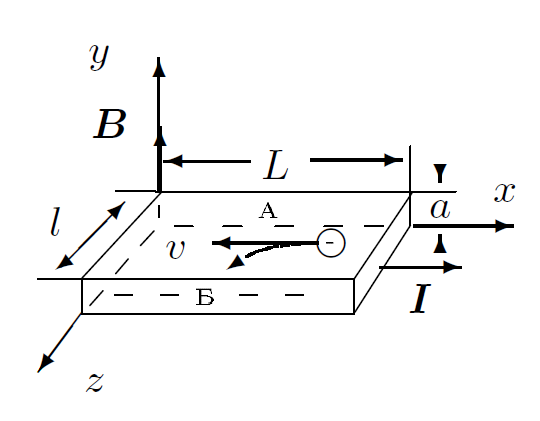
\includegraphics[width = 0.6\textwidth]{1.png}}\\
    \textit{Рис. 2: Эффект Холла}
\end{figure}

\noindent На электрон, движущийся в магнитном поле, действует сила Лоренца. Также на пластине с током, помещённой в магнитное поле, возникает разность потенциалов. В итоге, сила, действующая на электрон:

\begin{equation}
    F_1 = -eE - e<v>B
\end{equation}

\noindent Под действием этой силы электроны отклоняются к грани Б, на грани \linebreak А создаётся нескомпенсированный положительный заряд. Из-за разности потенциалов возникает электрическое поле, направленное от грани А к Б: $F_2 = eE_z$. Приравнивая $F_1$ и $F_2$, найдём ЭДС Холла:

\begin{equation}
    U_{ab} = - \frac{IB}{nea} = -R_x \frac{IB}{a}
\end{equation}

\noindent Также в эксперименте проводится измерение удельной проводимости образца:

\begin{equation}
    \sigma = \frac{I L_{35}}{U_{35} a l}
\end{equation}

\noindent Концентрация носителей тока в образце:

\begin{equation}
n = \frac{1}{R_\text{х} e}
\end{equation}

\noindent Подвижность носителей тока:

\begin{equation}
    b = \frac{\sigma}{en}
\end{equation}
